\subsection{Problem 4: Atap Seng di Siang Bolong}

\subsubsection{Identifikasi Masalah}

Sumber BMKG dan PVMBG bersifat diskret per kejadian dan diakses melalui HTTP \textit{polling} berkala. Sebaliknya, sumber \texttt{SATELIT} memancarkan aliran titik panas mentah secara kontinu lewat \textit{Server-Sent Events} (SSE). Satu titik panas tunggal bisa berasal dari atap seng di siang hari sehingga kebakaran baru terbentuk saat beberapa deteksi saling terhubung secara spasial dan temporal. Kondisi ini memunculkan lima persoalan utama:

\begin{enumerate}
  \item \textbf{Pengambilan data kontinu dengan risiko putus sambung dan duplikasi (Kriteria 1 dan 8).}
  Jika sistem tetap memakai \textit{periodic polling}, jeda antarpermintaan memperbesar latensi atau membuat kejadian terlewat saat \textit{stream} tidak menahan riwayat panjang tanpa kursor. Pada koneksi SSE panjang, gangguan jaringan atau \textit{restart} \textit{pod} juga dapat memutus aliran serta memicu celah atau duplikasi saat menyambung ulang. Dalam literatur, persoalan ini diselesaikan memakai \textbf{\textit{streaming ingestion with offset checkpointing}} dan \textbf{\textit{durable write-ahead feed log}}.

  \item \textbf{Ketidaksesuaian waktu tiba dengan waktu kejadian dan data terlambat (Kriteria 2).}
  Deteksi satelit tidak selalu tiba berurutan sesuai waktu pengamatan karena lintasan orbit sebelumnya dapat datang jauh lebih lambat. Mengelompokkan titik memakai jam sistem saat paket diterima (\textit{processing time}) akan menyatukan titik yang sebenarnya terpaut berjam-jam dan membuang titik sah yang datang belakangan. Persoalan ini dikenal sebagai \textbf{\textit{event-time versus processing-time skew}}, \textbf{\textit{out-of-order stream processing}}, serta \textbf{\textit{watermarks with bounded allowed lateness}}.

  \item \textbf{Klaster kebakaran dinamis akibat pembaruan dan pencabutan deteksi (Kriteria 1 dan 3).}
  Dua titik terhubung jika berjarak maksimal $1{,}0\text{ km}$ dan berselisih waktu paling lama $360\text{ menit}$ dengan \textit{confidence} bukan \texttt{low} (\texttt{'l'}). Suatu klaster minimal berisi dua anggota. Namun, deteksi yang masuk dapat menerima \textit{event} \texttt{update} (penurunan \textit{confidence} atau koreksi \texttt{frp}) maupun \texttt{retract}. Menghapus satu simpul penghubung dapat memecah klaster tanpa boleh melahirkan \texttt{HazardEvent} ganda, yang termasuk \textbf{\textit{dynamic connected-component maintenance}} dan \textbf{\textit{idempotent mutable upserts}}.

  \item \textbf{Lonjakan kecepatan aliran $60\times$ dari \textit{time-lapse} (Kriteria 4).}
  Pada percepatan $60\times$, satu menit waktu nyata mengalirkan satu jam data satelit secara beruntun. Menulis langsung ke basis data pada setiap kedatangan \textit{frame} akan memicu beban tulis berlebih sehingga \textit{backpressure} dapat memutus aliran SSE. Literatur menyebut persoalan ini sebagai \textbf{\textit{burst handling}}, \textbf{\textit{backpressure decoupling}}, dan \textbf{\textit{micro-batch effect coalescing}}.

  \item \textbf{Ketahanan \textit{state} pengklasteran sementara saat pemroses mengalami \textit{crash} (Kriteria 5).}
  Proses pengklasteran harus menjaga graf deteksi aktif yang masih berpeluang tersambung oleh titik berikutnya. Jika graf itu hanya hidup di RAM lalu \textit{pod} pemroses mati mendadak, seluruh klaster yang sedang tumbuh akan hilang atau membentuk nilai \texttt{fire\_id} berbeda setelah pulih. Persoalan ini disebut \textbf{\textit{stateful stream processing fault tolerance}}, yang diselesaikan melalui \textbf{\textit{checkpointing}} dan \textbf{\textit{deterministic replay}}.
\end{enumerate}

\subsubsection{Rancangan Solusi dan Mekanisme yang Dipilih}

Rancangan Problem 4 memisahkan tahap penangkapan aliran SSE ke log persisten dari tahap pengklasteran berbasis \textit{event time} beserta penulisan efek ke penyimpanan kanonik. Kedua tahap tersebut dikelola di bawah kepemimpinan tunggal \textit{lease} Kubernetes \texttt{aggregator-satellite} untuk sumber \texttt{SATELIT}. Alur lengkap arsitektur ditunjukkan pada \textbf{Gambar~\ref{fig:p4-arch}}.

\begin{figure}[H]
  \centering
  \IfFileExists{figures/p4-arsitektur-stream-satelit.png}{%
    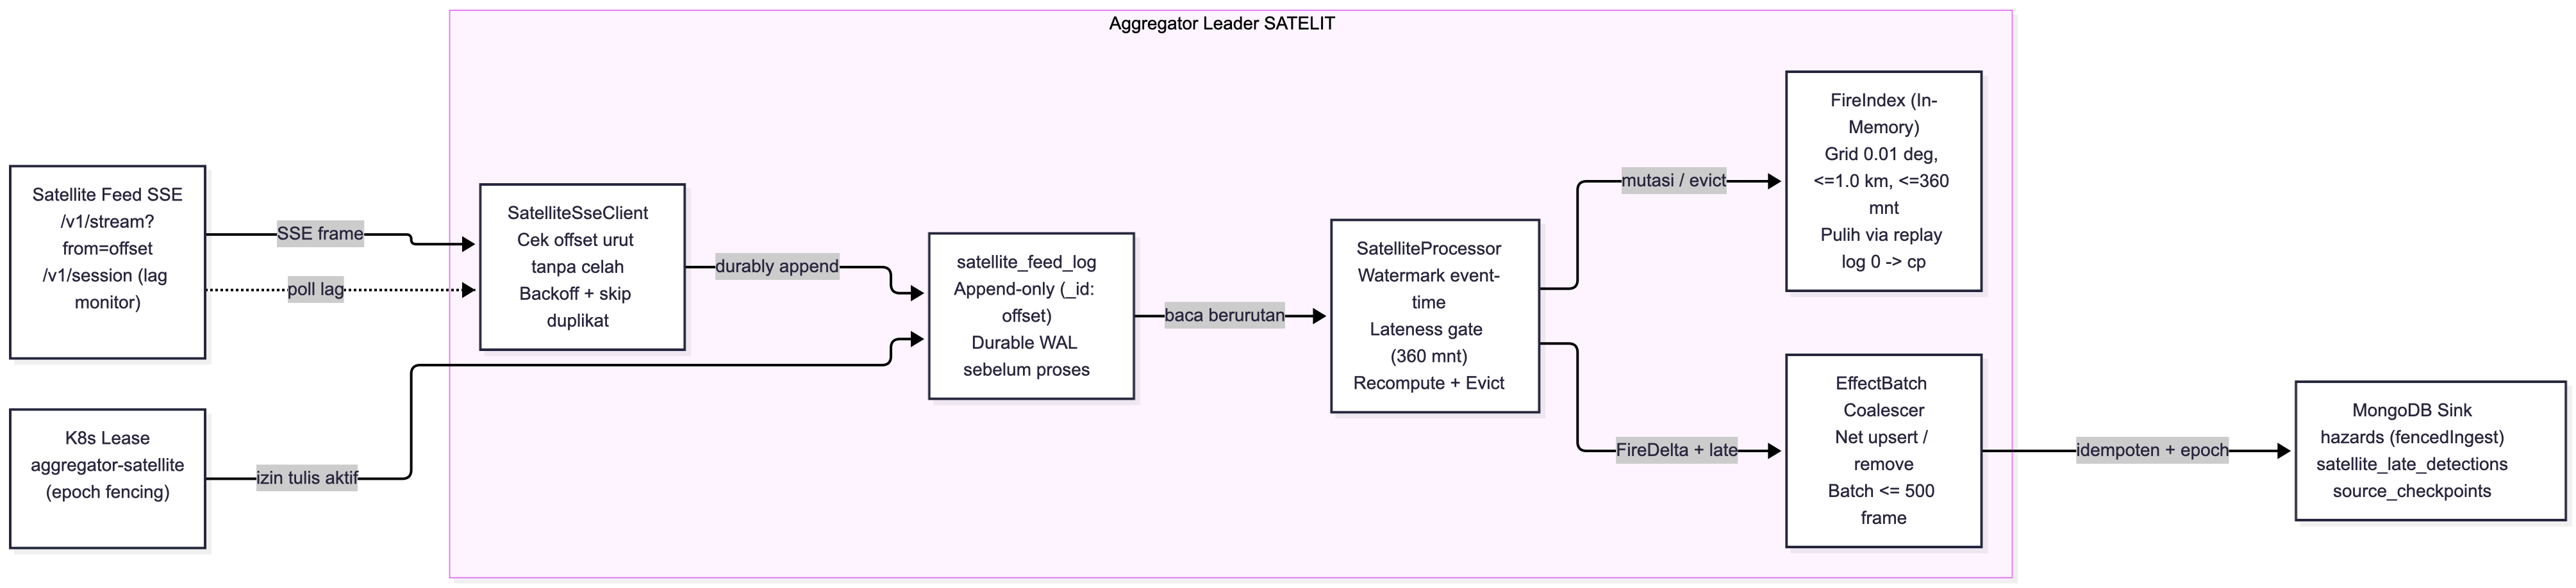
\includegraphics[width=0.95\linewidth]{p4-arsitektur-stream-satelit.png}%
  }{%
  \resizebox{\linewidth}{!}{%
  \begin{tikzpicture}[
    every node/.style={font=\sffamily\footnotesize},
    box/.style={draw=black!65, rounded corners=3pt, fill=white, align=center, inner sep=5pt, minimum width=3.1cm, minimum height=0.95cm},
    store/.style={draw=blue!55!black, rounded corners=2pt, fill=blue!6, align=center, inner sep=5pt, minimum width=3.2cm, minimum height=0.95cm},
    group/.style={draw=black!35, dashed, rounded corners=4pt, fill=black!2, inner sep=9pt},
    arr/.style={-{Stealth[length=2.2mm]}, thick, draw=black!75},
    lbl/.style={font=\sffamily\scriptsize, fill=white, inner sep=1.5pt, align=center}
  ]
    % Sumber & Koordinasi (kiri)
    \node[box] (feed)  at (0, 3.2) {\textbf{Satellite Feed SSE}\\{\scriptsize /v1/stream?from=offset}\\{\scriptsize /v1/session (lag monitor)}};
    \node[box] (lease) at (0, 0.2) {\textbf{K8s Lease}\\{\scriptsize aggregator-satellite}\\{\scriptsize (epoch fencing)}};

    % Ingestion Decoupling (kolom 2)
    \node[box]   (sse)     at (6.0, 3.2) {\textbf{SatelliteSseClient}\\{\scriptsize Cek offset urut tanpa celah}\\{\scriptsize Backoff + skip duplikat}};
    \node[store] (feedlog) at (6.0, 0.2) {\textbf{satellite\_feed\_log}\\{\scriptsize Append-only (\_id: offset)}\\{\scriptsize Durable WAL sebelum proses}};

    % Processor Stateful (kolom 3)
    \node[box] (proc) at (12.3, 3.2) {\textbf{SatelliteProcessor}\\{\scriptsize Watermark event-time}\\{\scriptsize Lateness gate ($360\text{ mnt}$)}\\{\scriptsize Recompute + Evict}};
    \node[box] (idx)  at (12.3, 0.2) {\textbf{FireIndex (In-Memory)}\\{\scriptsize Grid $0{,}01^\circ$, $\le 1{,}0\text{ km}$, $\le 360\text{ mnt}$}\\{\scriptsize Pulih via replay log $0 \to cp$}};

    % Sink & Checkpoint (kanan)
    \node[box]   (batch) at (18.6, 3.2) {\textbf{EffectBatch Coalescer}\\{\scriptsize Net upsert / remove}\\{\scriptsize Batch $\le 500$ frame}};
    \node[store] (mongo) at (18.6, 0.2) {\textbf{MongoDB Sink}\\{\scriptsize hazards (fencedIngest)}\\{\scriptsize satellite\_late\_detections}\\{\scriptsize source\_checkpoints}};

    % Grouping
    \begin{scope}[on background layer]
      \node[group, fit=(sse)(feedlog)(proc)(idx)(batch), label={[font=\sffamily\scriptsize\bfseries]above:Aggregator Leader SATELIT}] {};
    \end{scope}

    % Panah
    \draw[arr] ([yshift=3.5mm]feed.east) -- node[lbl, above] {SSE frame} ([yshift=3.5mm]sse.west);
    \draw[arr, dashed] ([yshift=-3.5mm]feed.east) -- node[lbl, below] {poll lag} ([yshift=-3.5mm]sse.west);
    \draw[arr] (sse) -- node[lbl, left] {durably append} (feedlog);
    \draw[arr] (lease) -- node[lbl, below] {izin tulis aktif} (feedlog);
    \draw[arr] (feedlog.north east) -- node[lbl, above, sloped] {baca berurutan} (proc.south west);
    \draw[arr] (proc) -- node[lbl, left] {mutasi / evict} (idx);
    \draw[arr] (proc) -- node[lbl, above] {FireDelta + late} (batch);
    \draw[arr] (batch) -- node[lbl, right] {idempoten + epoch} (mongo);
  \end{tikzpicture}%
  }%
  }
  \caption{Diagram Rancangan Solusi Pemrosesan Stream Satelit pada Problem 4}
  \label{fig:p4-arch}
\end{figure}

Secara terperinci, implementasi Problem 4 bertumpu pada lima mekanisme utama berikut.

\paragraph*{1. Konsumsi SSE Bebas Celah dan Pemisahan via Log Persisten}
Komponen \texttt{SatelliteSseClient} (\path{aggregator/src/satellite/feed/sseClient.ts}) menyambung ke \path{/v1/stream?from=<offset>} dengan kursor selalu dibaca ulang dari MongoDB lewat \texttt{resumeOffset()}. Setiap \textit{frame} ber-\textit{offset} lebih kecil dari \texttt{expected} dilewati sebagai duplikat. Jika muncul \textit{offset} lebih besar, klien memutus koneksi untuk menyambung ulang tepat pada posisi \texttt{expected}.

Ketika server membalas status \texttt{429} atau \texttt{503}, klien mematuhi \textit{header} \texttt{Retry-After} serta memakai \textit{exponential jittered backoff} hingga $15.000\text{ ms}$. Setiap \textit{frame} langsung disimpan oleh \texttt{createFeedIngestor} (\path{ingestor.ts}) ke koleksi \path{satellite_feed_log} (\texttt{\_id: offset}) sebelum diproses. Sementara itu, \texttt{runSessionMonitor} memantau \path{/v1/session} setiap 5 detik untuk mencatat \textit{offset lag}.

\paragraph*{2. Pengelompokan Spasial-Temporal dengan Indeks Grid dan Rekomputasi Lokal}
Kelas \texttt{FireIndex} (\path{aggregator/src/satellite/clustering/fireIndex.ts}) memisahkan titik ber-\textit{confidence} \texttt{'l'} agar tidak pernah menyambung klaster. Deteksi valid (\texttt{'n'} atau \texttt{'h'}) dipetakan ke petak \textit{grid} spasial $0{,}01^\circ$ sehingga pencarian tetangga hanya memeriksa $3 \times 3$ sel di sekitar titik terdampak.

Dua titik terhubung jika jarak \textit{Haversine} (\path{geo.ts}) maksimal $1{,}0\text{ km}$ dan selisih waktu maksimal $360\text{ menit}$. Pada tiap \texttt{detection}, \texttt{update}, atau \texttt{retract}, sistem menjalankan \textit{breadth-first search} lokal untuk menghitung ulang komponen terdampak. Komponen beranggotakan minimal dua titik membentuk \texttt{Fire} dengan \texttt{fire\_id} dari \textit{hash} titik paling awal dan keparahan \texttt{WASPADA}, \texttt{SIAGA}, atau \texttt{AWAS}. Hasil tersebut dipetakan menjadi \texttt{HazardEvent} bertipe \texttt{WILDFIRE}, sedangkan titik tunggal dicatat lewat \texttt{singletonCount}.

\paragraph*{3. \textit{Event-Time Watermark}, Batas Keterlambatan, dan Pembersihan Memori}
Kelas \texttt{Satellite\allowbreak Processor} (\path{aggregator/src/satellite/processing/processor.ts}) memajukan \texttt{watermarkMs} secara monotonik hanya dari \path{heartbeat.virtualNowMs} atau \path{detection.time_ms}. Deteksi dengan waktu lebih awal dari batas \texttt{watermarkMs} dikurangi \texttt{lateness\_ms} (\texttt{360 menit}) tidak dimasukkan ke klaster. Data tersebut dicatat secara \textit{idempotent} ke \path{satellite_late_detections} oleh \texttt{MongoLateStore} (\path{lateStore.ts}).

Setiap \texttt{1.000} \textit{offset}, pemroses memangkas komponen lama lewat \path{evictFinalized(cutoff)} pada batas $720\text{ menit}$ di belakang \textit{watermark} ($\texttt{lateness\_ms} + \texttt{MAX\_GAP\_MS}$). Langkah ini menjaga penggunaan memori tetap terbatas pada aliran jangka panjang tanpa mengorbankan ketepatan pengelompokan.

\paragraph*{4. Penggabungan Efek Batch dan Penulisan Ber-\textit{Epoch}}
Pemroses \texttt{run\allowbreak Satellite\allowbreak Processing} (\path{aggregator/src/satellite/processing/runner.ts}) membaca entri \path{satellite_feed_log} dalam kelompok hingga \texttt{500} \textit{frame}. Kelas \texttt{EffectBatch} menyatukan perubahan berulang atas \texttt{fire\_id} yang sama di dalam satu kelompok agar penyimpanan hanya menerima satu operasi bersih terakhir. Upsert memakai \texttt{fencedIngest} berversi \texttt{eventVersion:} \texttt{offset} dan \texttt{epoch}, sedangkan penghapusan memakai \texttt{repo.remove} setelah \textit{epoch} diverifikasi.

\paragraph*{5. Pemulihan \textit{State} via \textit{Replay} Deterministik}
Sesudah menulis efek dan catatan terlambat, pemroses menyimpan kemajuan ke \path{source_checkpoints} dengan nilai \texttt{committed\_offset}, \texttt{state\_version}, dan \texttt{owner\_epoch}. Ketika \textit{pod} mati atau kepemimpinan \texttt{aggregator-satellite} berpindah, pemimpin baru memutar ulang \path{satellite_feed_log} dari \textit{offset} \texttt{0} hingga \texttt{committed\_offset} memakai fungsi murni \texttt{proc.apply} tanpa efek samping. Cara ini memulihkan \texttt{FireIndex}, \texttt{watermarkMs}, dan daftar \texttt{retracted} secara identik sebelum memproses \textit{offset} berikutnya.

\subsubsection{Alasan Keputusan}

\textbf{Tabel~\ref{tab:p4-decisions}} merangkum pilihan desain utama Problem 4, alasan beserta implikasinya, dan alternatif yang ditolak.

\begin{small}
\begin{longtable}{@{} >{\raggedright\arraybackslash}p{3.4cm} >{\raggedright\arraybackslash}p{7.4cm} >{\raggedright\arraybackslash}p{4.0cm} @{}}
  \caption{Desain, Alasan, dan Alternatif yang Ditolak pada Problem 4}
  \label{tab:p4-decisions} \\
  \toprule
  \textbf{Keputusan} & \textbf{Alasan} & \textbf{Alternatif (Ditolak)} \\
  \midrule
  \endfirsthead
  \caption[]{Desain, Alasan, dan Alternatif yang Ditolak pada Problem 4 (Lanjutan)} \\
  \toprule
  \textbf{Keputusan} & \textbf{Alasan} & \textbf{Alternatif (Ditolak)} \\
  \midrule
  \endhead
  \midrule
  \multicolumn{3}{r}{\textit{Bersambung ke halaman berikutnya...}} \\
  \endfoot
  \bottomrule
  \endlastfoot
  Beralih ke klien SSE dengan log persisten \path{satellite_feed_log} & Sumber \texttt{SATELIT} memancarkan aliran kontinu ber-\textit{offset} urut. Menyimpan \textit{frame} mentah terlebih dahulu memisahkan kecepatan kedatangan jaringan (termasuk lonjakan $60\times$) dari laju olah klaster serta menjamin penyambungan ulang bebas celah. Konsekuensinya, log mentah memakai ruang disk MongoDB. & \textbf{\textit{Polling} periodik atau memproses SSE langsung di RAM:} rentan memutus koneksi akibat \textit{backpressure} saat lonjakan $60\times$ atau menghilangkan \textit{state} saat \textit{pod} mati. \\
  \midrule
  \textit{Event-time watermark} ($\max$ \texttt{virtual\_now} dan waktu deteksi) dengan \textit{lateness} $360\text{ menit}$ & Pada kecepatan $60\times$ dan kedatangan tak urut, jam sistem lokal gagal mencerminkan keterhubungan fisik kebakaran. Batas pembersihan $720\text{ menit}$ memastikan klaster usang aman dihapus. Konsekuensinya, titik lebih lambat dari $360\text{ menit}$ hanya dicatat sebagai \textit{late detection}. & \textbf{Pengelompokan berbasis \textit{processing time} atau tanpa pembersihan:} cara pertama memecah klaster sah saat kecepatan tinggi, sedangkan cara kedua memicu kebocoran memori. \\
  \midrule
  Rekomputasi BFS lokal pada \textit{grid} $0{,}01^\circ$ menggantikan \textit{Union-Find} & Peristiwa \texttt{update} ke \texttt{confidence = l} dan \texttt{retract} menghapus simpul maupun sisi sehingga klaster dapat terbelah. Petak \textit{grid} $0{,}01^\circ$ menjaga pencarian tetangga tetap cepat sementara BFS lokal menghitung ulang pemecahan klaster secara tepat. & \textbf{\textit{Disjoint-Set / Union-Find} standar:} efisien untuk penggabungan, tetapi tidak mendukung penghapusan sisi saat simpul penghubung ditarik kembali. \\
  \midrule
  Pemulihan pasca-\textit{crash} lewat \textit{replay} \path{satellite_feed_log} dan \textit{checkpoint} & \texttt{SatelliteProcessor} berjalan deterministik sehingga memutar ulang log hingga \texttt{committed\_offset} meniadakan kebutuhan serialisasi graf penuh di tiap \textit{batch}. Satu \textit{checkpoint} menjadi sangat ringan dan atomik. Konsekuensinya, lama waktu pemulihan sebanding dengan panjang log yang diputar ulang. & \textbf{Menyimpan seluruh \textit{snapshot} graf dan indeks \textit{grid} setiap \textit{batch}:} meningkatkan beban I/O tulis MongoDB secara tajam saat percepatan $60\times$. \\
  \midrule
  Penggabungan efek (\texttt{EffectBatch}) dan \texttt{eventVersion = offset} & Saat kecepatan $60\times$, satu kebakaran bisa berubah berkali-kali dalam satu kelompok \texttt{500 frame}. Penggabungan efek menekan drastis jumlah penulisan ke \texttt{hazards}, sementara \texttt{eventVersion} menjaga sifat \textit{idempotent} saat pemulihan. & \textbf{Menulis langsung ke MongoDB tiap satu deteksi masuk:} membanjiri basis data selama lonjakan $60\times$ dan melampaui batas latensi $60\text{ detik}$. \\
\end{longtable}
\end{small}

\subsubsection{Batasan yang Disadari}

\textbf{Tabel~\ref{tab:p4-limits}} mencatat batasan teknis yang disadari pada implementasi modul satelit.

\begin{table}[H]
  \centering
  \caption{Batasan Implementasi yang Disadari pada Problem 4}
  \label{tab:p4-limits}
  \small
  \begin{tabularx}{\linewidth}{@{} >{\raggedright\arraybackslash}p{3.6cm} >{\raggedright\arraybackslash}X >{\raggedright\arraybackslash}p{4.1cm} @{}}
    \toprule
    \textbf{Batasan} & \textbf{Penjelasan dan Alasan} & \textbf{Referensi Kode} \\
    \midrule
    \textbf{\textit{Replay} penuh dari \textit{offset} \texttt{0} tanpa \textit{snapshot} bawaan} & Pemulihan dasar memutar ulang log dari \textit{offset} \texttt{0} sampai \texttt{committed\_offset}. Untuk rentang uji Milestone 2 proses ini cepat, tetapi aliran bertahun-tahun memerlukan pemangkasan log atau penyimpanan \textit{snapshot} berkala agar waktu mulai tidak tumbuh linear. & \path{aggregator/src/satellite/processing/runner.ts} \\
    \midrule
    \textbf{Satu pemroses berpartisi tunggal} & Seluruh aliran \texttt{SATELIT} diproses pada partisi \texttt{'stream'} oleh satu pemegang \textit{lease} \texttt{aggregator-satellite}. Keterhubungan komponen dapat menyambung secara transitif lintas koordinat sehingga pembagian partisi paralel memerlukan penggabungan lintas batas. & \path{aggregator/src/satellite/service.ts}, \path{aggregator/src/satellite/clustering/fireIndex.ts} \\
    \midrule
    \textbf{Data terlambat di atas batas tidak membuka klaster} & Deteksi yang datang melewati $360\text{ menit}$ di belakang \textit{watermark} tidak dimasukkan ke \texttt{FireIndex}. Pembatasan ini sengaja dilakukan agar memori klaster usang bisa dibersihkan aman di batas $720\text{ menit}$, sementara catatannya tetap terekam unik di \path{satellite_late_detections}. & \path{aggregator/src/satellite/processing/processor.ts}, \path{aggregator/src/satellite/processing/lateStore.ts} \\
    \midrule
    \textbf{Penghentian \textit{batch} lama saat pindah kepemimpinan} & Bila \textit{pod} pemroses mati di antara \texttt{writeEffects} dan \texttt{commitCheckpoint}, \textit{batch} tersebut diulang oleh pemimpin baru. Pembaruan dengan \texttt{eventVersion} yang sama diabaikan oleh \texttt{fencedIngest} sehingga penulisan tetap aman. & \path{aggregator/src/satellite/processing/runner.ts}, \path{aggregator/src/coordination/fencing.ts} \\
    \bottomrule
  \end{tabularx}
\end{table}

\subsubsection{Bukti Penyelesaian per Kriteria}
\isian{Bagian ini akan diisi setelah eksekusi pengujian Problem 4 (\textit{streaming} langsung ke \path{https://satellite.naufarrel.dev}, simulasi percepatan $60\times$, penyuntikan \textit{crash} komponen pemroses saat klaster terbentuk, pemutusan koneksi SSE, serta verifikasi perbandingan terhadap hasil referensi asisten) selesai dijalankan di klaster.}

\begin{itemize}
  \item \textbf{Kriteria 1 (Pemetaan \textit{hotspot} $\to$ \texttt{HazardEvent WILDFIRE}):} \isian{Tampilkan hasil pengelompokan multisatelit menjadi satu \texttt{HazardEvent} dan pelaporan deteksi tunggal.}
  \item \textbf{Kriteria 2 (Pengelompokan berbasis \textit{event time} dan keterlambatan):} \isian{Tampilkan batas keterlambatan, pembaruan deteksi terlambat yang valid, dan jumlah deteksi melewati batas.}
  \item \textbf{Kriteria 3 (\textit{Update} dan \textit{retract}):} \isian{Tampilkan pembaruan \texttt{HazardEvent} eksisting tanpa menciptakan duplikat.}
  \item \textbf{Kriteria 4 (Percepatan $60\times$):} \isian{Tampilkan bukti 0 data hilang, waktu kejar $\le 60$ detik, $p_{95}$ latensi, dan \textit{lag} pada dasbor.}
  \item \textbf{Kriteria 5 (\textit{Crash} komponen pemroses saat pengenalan):} \isian{Tampilkan kesamaan hasil dengan pemrosesan tanpa gangguan.}
  \item \textbf{Kriteria 6 (Perbandingan hasil referensi asisten):} \isian{Tampilkan hasil \textit{checksum}/perbandingan dan penjelasan bila ada selisih.}
  \item \textbf{Kriteria 7 (Aliran \textit{live} beberapa menit):} \isian{Tampilkan tangkapan layar pemrosesan \textit{stream live}.}
  \item \textbf{Kriteria 8 (Putus dan menyambung ulang):} \isian{Tampilkan kelanjutan dari \textit{offset}/\texttt{Last-Event-ID} tanpa celah dan duplikat.}
\end{itemize}

\slotgambar{Bukti Penyelesaian Problem 4}{Bukti Pemrosesan Stream dan Perbandingan Referensi Problem 4}

\subsubsection{Jawaban atas Butir ``Di laporan''}

\paragraph*{Persoalan Aliran Waktu Kejadian, Lonjakan Kecepatan, dan Kegagalan Pemroses}
Ketiga kriteria kunci pada Problem 4 berkaitan erat dengan teori pemrosesan aliran (\textit{stream processing}). Kriteria 2 menyoroti ketimpangan antara waktu tiba paket dan waktu pengamatan fisik satelit yang tidak selalu urut. Dalam literatur, persoalan ini dikenal sebagai \textbf{\textit{event-time versus processing-time skew}} dan \textbf{\textit{out-of-order stream processing}}, yang ditangani memakai \textbf{\textit{watermarks with bounded allowed lateness}}.

Kriteria 4 memunculkan lonjakan laju kedatangan $60\times$ yang mengancam kestabilan I/O penyimpanan maupun koneksi jaringan. Persoalan ini disebut \textbf{\textit{backpressure}} dan diselesaikan lewat pemisahan produsen dan konsumen berbasis log persisten serta penggabungan efek per \textit{batch}. Sementara itu, Kriteria 5 menghadapi risiko hilangnya graf pengklasteran saat \textit{pod} mati di tengah proses, yang dikenal sebagai \textbf{\textit{stateful stream processing fault tolerance}}.

\paragraph*{Mengapa Pola \textit{Polling} Milestone 1 Ditinggalkan}
Untuk sumber \texttt{SATELIT}, pola \textit{periodic polling} dari Milestone 1 ditinggalkan dan digantikan oleh konsumsi \textit{streaming} SSE di atas \texttt{MongoFeedLog}. Sumber satelit mengekspos aliran kontinu pada \path{/v1/stream?from=<offset>} berurutan tanpa celah, bukan daftar kondisi statis per siklus seperti BMKG atau PVMBG.

Pada mode percepatan $60\times$, \textit{polling} berkala tiap beberapa detik akan menumpuk perubahan sekaligus atau tertinggal mengejar progres peristiwa secara bertahap. Memakai SSE berbasis \textit{offset} memungkinkan sistem menyambung ulang instan setelah putus tanpa kehilangan data maupun mengolah ulang masa lalu. Endpoint \path{/v1/session} kini hanya dipantau ringan tiap 5 detik untuk menampilkan metrik ketertinggalan (\textit{offset lag}) di dasbor.

\paragraph*{Finalisasi Klaster, Data Terlambat, dan Ketahanan \textit{State}}
Secara inkremental, komponen pada \texttt{FireIndex} langsung diterbitkan ke \texttt{hazards} begitu memiliki minimal dua deteksi dan terus diperbarui setiap ada penambahan anggota, \texttt{update}, maupun \texttt{retract}. Sebuah kebakaran dinyatakan \textbf{selesai dikenali secara permanen} dan dihapus dari memori (\texttt{evictFinalized}) setelah waktu deteksi terakhirnya tertinggal di belakang batas \texttt{watermarkMs - lateness\_ms - MAX\_GAP\_MS}. Dengan baku masing-masing $360\text{ menit}$, titik aman berada $720\text{ menit}$ di belakang \textit{watermark} sehingga tidak ada lagi deteksi sah yang dapat menyambung komponen tersebut.

Selama kedatangan deteksi terlambat masih berada dalam rentang $\le 360\text{ menit}$ di belakang \textit{watermark}, titik tersebut tetap diterima penuh ke dalam \texttt{FireIndex} dan memperbarui dokumen \texttt{HazardEvent} tanpa duplikasi. Jika datang melewati batas $360\text{ menit}$, deteksi tidak memodifikasi klaster lama, melainkan menaikkan metrik \path{satellite_late_detections} dan dicatat unik pada koleksi MongoDB \path{satellite_late_detections}.

Agar tahan terhadap Kriteria 5, seluruh \textit{frame} mentah dipersistenkan berurutan ke koleksi \path{satellite_feed_log} terlebih dahulu, sedangkan kemajuan \textit{batch} disimpan di \path{source_checkpoints}. Graf \texttt{FireIndex}, \texttt{watermarkMs}, dan set \texttt{retracted} cukup berjalan di memori agar komputasi cepat. Bila \textit{pod} mati mendadak, pemimpin baru memutar ulang \path{satellite_feed_log} dari awal hingga \texttt{committed\_offset} secara deterministik sebelum memproses \textit{batch} berikutnya.

\paragraph*{Jaminan Pemrosesan Akhir}
Sistem mencapai jaminan \textbf{\textit{effectively-once state semantics}} pada penyimpanan akhir MongoDB \texttt{hazards} dan \path{satellite_late_detections}. Jaminan ini berdiri di atas penerimaan SSE minimal sekali bebas celah oleh \texttt{SatelliteSseClient} bersama \texttt{MongoFeedLog} (\texttt{\_id: offset}).

Apabila pemroses mati tepat di antara penulisan efek dan pembaruan \textit{checkpoint}, pemimpin baru akan mengulang \textit{batch} pasca-\texttt{committed\_offset}. Penulisan ulang ke \texttt{hazards} ditahan oleh \texttt{fencedIngest} lewat parameter \texttt{eventVersion: offset} dan \texttt{epoch}, sedangkan catatan terlambat ditahan kunci \texttt{\_id: r.key} di \texttt{MongoLateStore}. Dengan mekanisme ini, kondisi akhir kebakaran, jumlah titik panas, nilai FRP, serta jumlah deteksi tunggal dan terlambat pasca-\textit{crash} tetap identik dengan eksekusi tanpa gangguan.
